\chapter{美国流感住院数据实证}
\label{chap:empirical}

第三章给出的方差结构 $v_R+A/m$ 有一个可以在数据中检验的推论：在环境围绕同一均值波动的时段内，增长统计量的相对误差应当随规模下降，并趋于一个与规模无关的常数。第四章的更新过程仿真进一步说明，在时间序列中检验这一形状时，横轴应取实际规模 $D_t$，单代公式只能作参照曲线。本章用美国国家医疗安全网络的州级流感住院周报检验这一形状。第~\ref{sec:emp-data}~节说明数据、规模测度与填报制度分期。第~\ref{sec:emp-method}~节给出误差指标与估计方法。第~\ref{sec:emp-early}~节报告流行初期的规模效应。第~\ref{sec:emp-inflation}~节分析拟合截距与斜率高于理论值的原因。第~\ref{sec:emp-peak}~节与第~\ref{sec:emp-policy}~节分别考察流行达峰和填报制度变化时误差形状的变化。替代设定、空间汇总与外部数据留在第六章。

\section{数据与变量}
\label{sec:emp-data}

\subsection{数据来源与样本}

数据来自美国国家医疗安全网络（National Healthcare Safety Network，NHSN）公布的各辖区每周实验室确诊流感住院数，以及各辖区填报医院所占的比例\citep{cdc2026nhsn}。样本覆盖 50 个州与华盛顿特区，共 51 个辖区，时间从 2020 年 10 月至 2026 年 9 月，合计 16,218 个州周。其中 504 个州周的住院数缺失，468 个在下文的第一期，36 个在第二期。缺失按 0 处理。这一处理在强制填报期影响很小，在自愿填报期则可能把未填报误记为零住院，第~\ref{sec:emp-policy}~节解读第二期结果时会回到这一点。

选择住院数据首先是因为住院是流感监测中口径最稳定、报告最及时的指标之一，各州按统一定义每周上报，适合作跨辖区比较。此外，住院占感染的比例很低，文献估计在 0.0056--0.021 之间\citep{zhou2012hospitalizations, tokars2018seasonal}。按第三章命题~\ref{prop:reporting} 的数量分析，此时扩大覆盖与提高报告率的边际效果几乎相同，规模项主要由报告抽样决定，模型结构相对简单。

\subsection{规模测度与增长统计量}

第四章式~\eqref{eq:dt} 把规模定义为此前各周报告数按世代间隔加权的和。实证中取三周权重
\begin{equation}
  D_t=0.65\,C_t+0.25\,C_{t-1}+0.10\,C_{t-2},
  \label{eq:dt-main}
\end{equation}
其中 $C_t$ 为第 $t$ 周的住院数。相对于待预测的 $C_{t+1}$，三项的滞后分别为 1、2、3 周，平均回溯滞后为 $0.65\times1+0.25\times2+0.10\times3=1.45$ 周，约 10.2 天。权重集中在最近一周，与流感序列间隔短于一周的证据相符\citep{cowling2009estimation, vink2014serial}；第~\ref{sec:emp-inflation}~节比较另外两种权重。增长统计量取 $G_t=C_{t+1}/D_t$。小规模时 $G_t$ 的分母接近零，比值极不稳定，因此只保留 $D_t\geq5$ 的州周，得到 10,303 个有效观测。

$G_t$ 与第三章的 $R_t$ 不是同一个量。流感的世代间隔约 3 天，一周约跨两代传播，$G_t$ 是两代左右增长的合成，其均值与方差都不等于单代再生数的均值与方差。实证检验因而只使用模型的结构，即相对误差随规模变化的形状；拟合得到的系数描述的是 $G_t$ 这一统计量的误差，不解读为单代参数 $v_R$ 与 $A$ 的估计。这一区分贯穿本章和第六章。

\subsection{填报制度分期}

样本期内 NHSN 的填报制度变过两次。2020 年 10 月至 2024 年 4 月 30 日为强制填报，下称第一期。2024 年 5 月 1 日至 10 月 31 日改为自愿填报，下称第二期。2024 年 11 月 1 日起，美国联邦医疗保险与医疗补助服务中心恢复强制要求，下称第三期。表~\ref{tab:policy} 列出三期的样本量与填报率。第一期与第三期的平均填报率都在 91\% 以上。第二期降到 54.6\%，中位数只有 45.7\%，约一半辖区的填报医院不足半数。

\begin{table}[!tbp]
  \centering
  \caption{三个填报制度期的样本与周增长比的分布特征}
  \label{tab:policy}
  \begin{tabular}{@{}lccc@{}}
    \toprule
    指标 & 第一期（强制） & 第二期（自愿） & 第三期（恢复强制） \\
    \midrule
    有效州周数 & 6,009 & 420 & 3,874 \\
    平均填报率（\%） & 91.1 & 54.6 & 91.8 \\
    填报率中位数（\%） & 92.3 & 45.7 & 93.2 \\
    $G_t$ 均值 & 1.066 & 0.966 & 1.084 \\
    $G_t$ 标准差 & 0.624 & 1.823 & 0.649 \\
    $G_t$ 四分位距 & 0.638 & 0.594 & 0.652 \\
    $G_t$ 中位绝对偏差 & 0.298 & 0.299 & 0.292 \\
    $G_t$ 第 10 百分位数 & 0.468 & 0.199 & 0.508 \\
    $G_t$ 第 90 百分位数 & 1.772 & 1.459 & 1.914 \\
    $G_t$ 偏度 & 3.29 & 14.98 & 2.68 \\
    $G_t$ 最大值 & 12.7 & 33.9 & 11.5 \\
    \bottomrule
  \end{tabular}

  \vspace{4pt}
  {\small 注：有效州周指 $D_t\geq5$ 的州周；三期的有效州周合计 10,303 个。}
\end{table}

图~\ref{fig:nhsn} 画出全国周住院合计与平均填报率。住院数呈明显的季节性，每年 10 月前后开始上升，12 月至次年 2 月达峰，三个流行季的峰高逐季增加。填报率在第二期断崖式下降，第三期恢复后与第一期相当。图中绿色区间是第~\ref{sec:emp-early}~节使用的流行初期窗口，三个窗口都落在强制填报期内，窗口内的数据不受第二期填报率下降的影响。

\begin{figure}[!tbp]
  \centering
  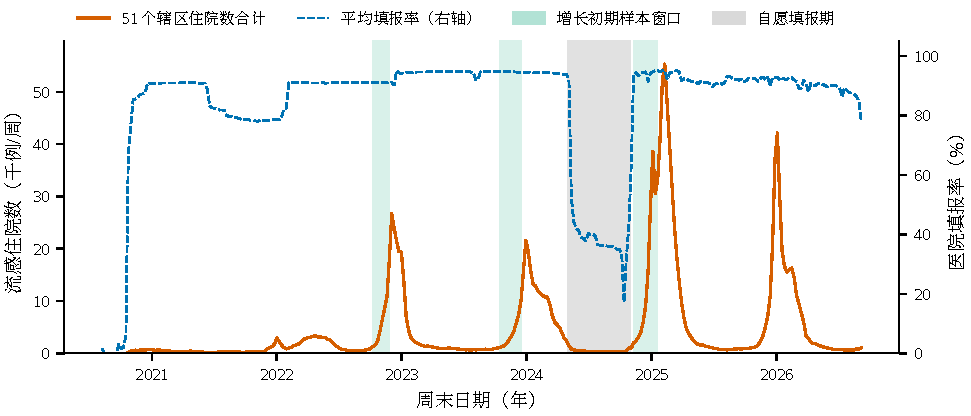
\includegraphics[width=\textwidth]{figures/fig_5_1_nhsn_series.pdf}
  \caption{美国 51 个辖区每周流感住院数合计（实线，左轴）与医院平均填报率（虚线，右轴）。缺失按 0 计入合计；绿色区间为三个流行季的增长初期样本窗口，灰色区间为 2024 年 5--10 月的自愿填报期。}
  \label{fig:nhsn}
\end{figure}

\section{误差指标与估计方法}
\label{sec:emp-method}

\subsection{相对均方误差}

误差指标采用相对均方误差。以某一阶段的平均增长比 $\Rbar$ 为基准，第 $t$ 周的损失定义为
\begin{equation}
  L_t=\Bigl(\frac{G_t-\Rbar}{\Rbar}\Bigr)^2 .
  \label{eq:loss}
\end{equation}
由第四章式~\eqref{eq:identity}，$L_t$ 也是用 $\Rbar D_t$ 预测 $C_{t+1}$ 的相对误差平方，属于预测评价中常用的相对误差评分\citep{bosse2023scoring}。这一恒等关系使下文可以在预测与估计两种读法之间切换。作为预测误差，$L_t$ 衡量以阶段均值外推一周的准确程度。作为估计误差，$L_t$ 衡量单周增长比偏离阶段均值的程度，对应目标Ⅱ。

在单代模型下，以预计报告规模 $m$ 代替 $D_t$，由命题~\ref{prop:average} 两边同除以 $\Rbar^2$，得到损失的条件期望
\begin{equation}
  \E(L_t\mid D_t)\approx a+\frac{b}{D_t},\qquad a=\frac{v_R}{\Rbar^2},\quad b=\frac{A}{\Rbar^2},\quad \frac ba=\mx .
  \label{eq:affine}
\end{equation}
式~\eqref{eq:affine} 是本章的拟合形式。截距 $a$ 对应环境底板，斜率 $b$ 对应规模项，比值 $b/a$ 称为经验交叉点。第四章第~\ref{sec:design-renewal}~节已经说明，在时间序列中 $D_t$ 只是 $\rho\Lambda_{t+1}$ 的带噪代理，式~\eqref{eq:affine} 的第一项与单代公式未必相等，条件偏差项也不为零。因此式~\eqref{eq:affine} 在这里是一个检验形状的工作模型，其系数是否等于 $v_R/\Rbar^2$ 与 $A/\Rbar^2$ 需要单独分析。

\subsection{可行广义最小二乘与聚类重抽}

损失的方差随规模变化。规模小时，$G_t$ 的分母噪声大，损失分布高度右偏；规模大时，损失集中在截距附近。普通最小二乘对所有观测等权，小规模观测的大方差会主导拟合。为此采用可行广义最小二乘\citep{wooldridge2010econometric}：第一步用普通最小二乘得到拟合值 $\hat\mu_t=\hat a+\hat b/D_t$；第二步以 $1/\hat\mu_t^2$ 为权重重新拟合。若损失近似服从变异系数恒定的分布，其方差与均值的平方成正比，$1/\hat\mu_t^2$ 即为近似最优权重。

区间估计采用按州聚类的自助法\citep{cameron2008bootstrap, cameron2015practitioner}。同一州相邻各周的损失相关，按州整体重抽可以保留州内的时间相关结构。重抽 1,500 次，每次重复两步估计，取 2.5\% 与 97.5\% 分位数作为 95\% 区间。经验交叉点的区间由每次重抽的 $\hat b/\hat a$ 直接取分位数，不依赖比值的正态近似。分箱均值的区间同样由按州聚类的重抽给出。

\section{流行初期的规模效应}
\label{sec:emp-early}

\subsection{样本窗口}

模型假定各期环境围绕同一均值波动。流行初期病例持续增长，传播水平相对稳定，最接近这一情形，所以主分析取三个流行季的增长初期，即 2022 年 10 月 8 日至 11 月 26 日、2023 年 10 月 14 日至 12 月 16 日、2024 年 11 月 9 日至 2025 年 1 月 18 日。窗口内共 1,267 个有效州周，平均增长比 $\Rbar_{\mathrm{early}}=1.6706$，标准差 0.7116。平均增长比大于 1，说明窗口内住院数平均每周增长约三分之二。2020--2021 和 2021--2022 两季受 2019 冠状病毒病大流行期间防控措施的影响，流感活动低且不规则，没有纳入初期窗口。

\subsection{分箱结果}

表~\ref{tab:early-bins} 按 $D_t$ 把初期样本分为六箱。平均损失从最小箱的 0.329 降到 $[20,50)$ 箱的 0.160，再降到 $[100,250)$ 箱的 0.112，此后两箱停在 0.103 和 0.105 附近，后三箱的 95\% 区间相互重叠。误差先随规模快速下降、再趋于平缓，这正是“常数加规模反比”的形状。各箱的中位数比均值小得多，最小箱的中位数只有 0.097，说明损失分布右偏，少数极端周拉高了均值。

\begin{table}[!tbp]
  \centering
  \caption{流行初期按实现规模分箱的平均损失}
  \label{tab:early-bins}
  \begin{tabular}{@{}lcccccc@{}}
    \toprule
    $D_t$ 分箱 & 州周数 & 州数 & 平均损失 & 95\% 区间 & 中位数 & $\Var(L)/\E(L)^2$ \\
    \midrule
    $[5,20)$ & 319 & 41 & 0.329 & 0.244--0.415 & 0.097 & 5.32 \\
    $[20,50)$ & 297 & 48 & 0.160 & 0.124--0.197 & 0.060 & 3.31 \\
    $[50,100)$ & 187 & 48 & 0.145 & 0.106--0.184 & 0.048 & 3.38 \\
    $[100,250)$ & 220 & 41 & 0.112 & 0.090--0.134 & 0.055 & 2.12 \\
    $[250,600)$ & 152 & 36 & 0.103 & 0.077--0.129 & 0.046 & 1.35 \\
    $[600,5000)$ & 92 & 20 & 0.105 & 0.077--0.134 & 0.074 & 0.99 \\
    \bottomrule
  \end{tabular}

  \vspace{4pt}
  {\small 注：95\% 区间由按州聚类的重抽得到；最后一列为箱内损失方差与均值平方之比。}
\end{table}

图~\ref{fig:early} 把分箱均值画在箱内平均 $D_t$ 处，并叠加式~\eqref{eq:affine} 的拟合曲线。拟合曲线穿过全部六个分箱的区间，左端随 $1/D_t$ 陡降，右端贴近截距虚线。经验交叉点位于第二箱附近，即规模达到每周二十余例时，截距与规模项各占一半。

\begin{figure}[!tbp]
  \centering
  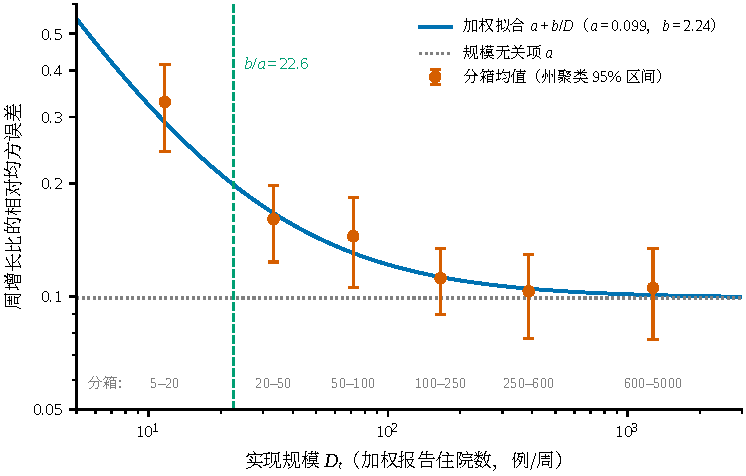
\includegraphics[width=0.8\textwidth]{figures/fig_5_2_early_scale.pdf}
  \caption{流行初期单步预测误差随实现规模 $D_t$ 的变化，共 1,267 个州周。圆点为各分箱均值，画在箱内平均 $D_t$ 处，误差棒为按州聚类重抽的 95\% 区间；曲线为 $a+b/D$ 的拟合，水平虚线为截距 $a$，竖线为经验交叉点 $b/a$。}
  \label{fig:early}
\end{figure}

\subsection{仿射模型的估计}

表~\ref{tab:affine} 汇总主估计与几种估计口径。主估计为 $a=0.0991$（95\% 区间 0.0841--0.1173），$b=2.2434$（1.5019--3.0161），1,500 次重抽中没有一次 $b\leq0$。经验交叉点 $b/a=22.6$ 例/周，区间为 13.7--33.7。用十分位分组均值代替逐观测拟合，交叉点同样为 22.6，说明主估计不依赖分箱方式。

\begin{table}[!tbp]
  \centering
  \caption{流行初期仿射误差模型的估计}
  \label{tab:affine}
  \small
  \begin{tabular}{@{}lccc@{}}
    \toprule
    估计口径 & 截距 $a$ & 斜率 $b$ & 经验交叉点 $b/a$ \\
    \midrule
    可行广义最小二乘（主估计） & 0.0991（0.0841--0.1173） & 2.243（1.502--3.016） & 22.6（13.7--33.7） \\
    十分位分组均值拟合 & 0.1006 & 2.271 & 22.6 \\
    普通最小二乘 & -- & 2.305 & -- \\
    剔除损失最大的 1\% & 0.1077（0.0913--0.1260） & 1.137（0.697--1.661） & 10.6（5.9--17.3） \\
    重抽时重估基准 $\Rbar_{\mathrm{early}}$ & （0.0843--0.1160） & （1.517--2.981） & -- \\
    按周聚类重抽 & （0.0611--0.1317） & （1.473--3.119） & -- \\
    \bottomrule
  \end{tabular}

  \vspace{4pt}
  {\small 注：括号内为 95\% 区间；后两行只改变推断方式，点估计同主估计。各口径下所有重抽的 $b$ 均为正。}
\end{table}

权重的选择只影响效率，不影响一致性。表~\ref{tab:early-bins} 最后一列显示，$\Var(L)/\E(L)^2$ 从最小箱的 5.32 降到最大箱的 0.99，损失的变异系数并不恒定，所以 $1/\hat\mu^2$ 并非最优权重。权重只依赖 $D_t$，与误差项无关，拟合仍然一致；普通最小二乘给出 $b=2.305$，与 2.243 接近。

交叉点对极端值敏感。去掉损失最大的 1\% 观测后，$a$ 升到 0.1077，$b$ 降到 1.137，交叉点降到 10.6。极端损失集中在小规模州周，剔除后斜率下降最多，截距几乎不变。这说明经验交叉点的位置在相当程度上取决于小规模处的尾部行为，下文只把它当作量级。推断方式的两项变化不改变结论。每次重抽都重新估计基准 $\Rbar_{\mathrm{early}}$ 时，$b$ 的 95\% 区间为 1.517--2.981；按周聚类时为 1.473--3.119。州与周两个维度的双向聚类没有做，原因见第~\ref{sec:concl-limits}~节。

\subsection{误差预算与反事实规模}

把平均损失拆开，可以看出扩大规模还剩多少空间。初期样本的平均损失为 0.181，其中截距 $a$ 占 54.6\%，规模项 $b/D_t$ 占 45.1\%，拟合残差占 0.2\%；规模项按 $D_t$ 的调和平均数 27.4 计算。调和平均数接近经验交叉点 22.6，所以两部分大致各占一半，与命题~\ref{prop:average}(ii) 在 $m\approx\mx$ 处的结论一致。

若所有州周的规模都提高到每周 250 例，模型给出的平均损失为 0.107，比现状下降 40.9\%。剩下的 0.107 中，截距 0.0991 占九成以上，继续扩大规模的回报已经很小。实际 $D_t\geq250$ 的 244 个州周，平均损失为 0.104，约为全样本均值的 57\%，与模型给出的 $a+b/250=0.108$ 接近。后一个吻合由拟合机械地决定，大规模观测本身参与了拟合，因此只说明模型在大规模一端没有明显失配，不构成独立证据。

\subsection{与理论情景区间的比较}

经验交叉点 22.6 与理论情景区间处于同一量级。情景参数取 $\Rbar=1.67$，$k\in[0.2,0.5]$\citep{lloydsmith2005superspreading}，$\rho\in[0.0056,0.021]$\citep{zhou2012hospitalizations, tokars2018seasonal}，$v_R\in[0.04,0.08]$。由式~\eqref{eq:var-average}，此时 $A$ 在 1.702--1.967 之间，交叉点 $\mx$ 在 21.3--49.2 之间。报告率很低，$A$ 中的超传播项 $\rho(\Rbar^2+v_R)/k$ 至多约 0.3，$A$ 主要由 $\Rbar$ 决定，交叉点的变化主要来自 $v_R$。

比值落入区间不能当作对结构参数的检验。情景隐含的截距 $v_R/\Rbar^2$ 为 0.0143--0.0287，斜率 $A/\Rbar^2$ 为 0.610--0.705；实证 $a$ 是前者的 3.5--6.9 倍，$b$ 是后者的 3.2--3.7 倍。截距与斜率都被放大了数倍，放大倍数相近，比值才落在区间内。若两者的放大倍数不同，经验交叉点可以远离情景区间，而误差形状本身不变。第~\ref{sec:emp-inflation}~节分析两类放大的来源。

\section{截距与斜率偏大的来源}
\label{sec:emp-inflation}

截距与斜率高于情景隐含值，有两个来源分别作用于斜率和截距。斜率的放大主要来自分母中的报告噪声；截距的放大与环境的时间相关以及 $G_t$ 的口径有关。

\subsection{分母噪声与斜率}

$D_t$ 本身是带二项报告噪声的计数，比真实感染压力 $\rho\Lambda_{t+1}$ 多一层随机性。第四章第~\ref{sec:design-renewal}~节在仿真中已经看到，$D_t$ 偶然偏小时 $G_t$ 被放大，而 $1/D_t$ 是凸函数，对称的分母噪声会抬高平均误差。用 delta 方法展开到 $1/m$ 阶，斜率近似为
\begin{equation}
  b\approx\frac{A+(1-\rho)(\Rbar^2+v_R)\sum_s {w_s}^2}{\Rbar^2},
  \label{eq:b-delta}
\end{equation}
其中 $\sum_s {w_s}^2$ 是式~\eqref{eq:dt-main} 中滞后权重的平方和。式~\eqref{eq:b-delta} 的推导及其成立条件见附录~\ref{app:b-delta}。分子第二项是分母噪声的贡献。住院比例 $\rho$ 很小，$1-\rho$ 接近 1，噪声几乎完整地保留下来；权重越集中，$D_t$ 越接近单周计数，$\sum_s {w_s}^2$ 越大，斜率也越大。分母或自变量含噪时回归系数发生偏移，是测量误差文献中的经典问题\citep{fuller1987measurement, carroll2006measurement}。

式~\eqref{eq:b-delta} 给出一个可检验的预测：改变滞后权重时，斜率应按 $\sum_s {w_s}^2$ 同向变化。表~\ref{tab:lag-weights} 比较三种权重，即主规格（0.65/0.25/0.10，$\sum w^2=0.495$）、只用当周（$\sum w^2=1$）和三周等权（$\sum w^2=0.333$）。实证斜率依次为 2.243、3.134（95\% 区间 2.203--4.067）和 1.926（1.071--2.807），顺序与 $\sum w^2$ 一致。相对主规格，后两者的比值为 1.40 和 0.86；式~\eqref{eq:b-delta} 在情景参数下的预测为 1.44 和 0.86，二者相当接近。三种权重下的 $\Rbar$ 不同（1.48、1.67、1.99），比值的吻合只作方向与量级的对照。

\begin{table}[!tbp]
  \centering
  \caption{三种滞后权重下的实证拟合与情景模拟}
  \label{tab:lag-weights}
  \small
  \begin{tabular}{@{}lccccccc@{}}
    \toprule
    \multirow{2}{*}{规格} & \multirow{2}{*}{$\sum w^2$} & 平均滞后 & \multicolumn{3}{c}{实证} & \multicolumn{2}{c}{情景（$b$）} \\
    \cmidrule(lr){4-6}\cmidrule(l){7-8}
     & & （周） & $a$ & $b$ & $b/a$ & 式~\eqref{eq:b-delta} & 模拟 \\
    \midrule
    只用当周 & 1.000 & 1.00 & 0.0682 & 3.134 & 46.0 & 1.660 & 1.566 \\
    主规格 & 0.495 & 1.45 & 0.0991 & 2.243 & 22.6 & 1.155 & 1.195 \\
    三周等权 & 0.333 & 2.00 & 0.1524 & 1.926 & 12.6 & 0.993 & 0.999 \\
    \bottomrule
  \end{tabular}

  \vspace{4pt}
  {\small 注：情景参数为 $\overline{R}=1.67$，$v_R=0.06$，$k=0.35$，$\rho=0.021$，$A=1.8409$；没有分母噪声时情景斜率为 0.660。模拟以样本均值归一化，每种权重 18,000 个模拟州周。}
\end{table}

情景模拟进一步核对了式~\eqref{eq:b-delta}。情景参数取 $\Rbar=1.67$，$v_R=0.06$，$k=0.35$，$\rho=0.021$，$A=1.8409$。三种权重的预测斜率为 1.155、1.660、0.993，模拟值为 1.195、1.566、0.999。只用当周权重时模拟值低于预测约 6\%，此时分母噪声最大，含噪回归元的稀释、$D_t\geq5$ 的截断与小规模处的高阶余项都更明显，附录~\ref{app:b-delta} 讨论了这三者的方向。图~\ref{fig:noise}a 把实证估计、模拟值与式~\eqref{eq:b-delta} 的直线画在一起，三者随 $\sum w^2$ 同向上升。

在水平上，分母噪声只解释了实证斜率的一部分。没有分母噪声时，情景斜率为 0.660，约为实证值的 29\%；加入二项分母噪声后升到 1.155，约为 51\%。剩余部分的一个可能来源是报告过程的超额离散：若报告数的方差是二项方差的 $\varphi$ 倍，取 $\varphi=1.96$ 时模拟斜率为 2.019，接近实证水平。这只是可能的解释之一，现有数据无法区分超额离散与其他来源，例如各州住院比例的差异。

\subsection{分母噪声不抬高截距}

分母噪声只进入 $1/m$ 阶，不改变截距。情景模拟中主规格、只用当周与三周等权的截距为 0.0202、0.0225、0.0214，几乎不变，都接近 $v_R/\Rbar^2=0.0215$。斜率被放大而截距不变，于是 $b/a$ 被推高。主规格的模拟比值为 59.2，而真实的 $A/v_R$ 只有 30.7。用经验交叉点估计 $\mx$ 因而会系统性偏大。实证中 $b/a$ 没有偏大到这一程度，是因为实证截距也被放大了，两种放大部分抵消。

\subsection{截距随回溯滞后上升}

截距的放大另有来源。表~\ref{tab:lag-weights} 中实证截距随平均回溯滞后单调上升，平均滞后为 1.0、1.45、2.0 周时，$a$ 分别为 0.0682、0.0991、0.1524，都远高于情景隐含的 0.014--0.029（图~\ref{fig:noise}b）；模拟中截距不随滞后变化。这一模式与第四章式~\eqref{eq:mse-decomp} 的条件偏差项一致。真实的 $R_t$ 有时间相关，分母越陈旧，$\mu_t/D_t$ 偏离 $\Rbar$ 越远，偏差项越大。$G_t$ 跨两代左右，代际之间的环境波动叠加，也会放大与规模无关的部分。两种机制都作用于截距，现有数据无法把它们分开。

\begin{figure}[!tbp]
  \centering
  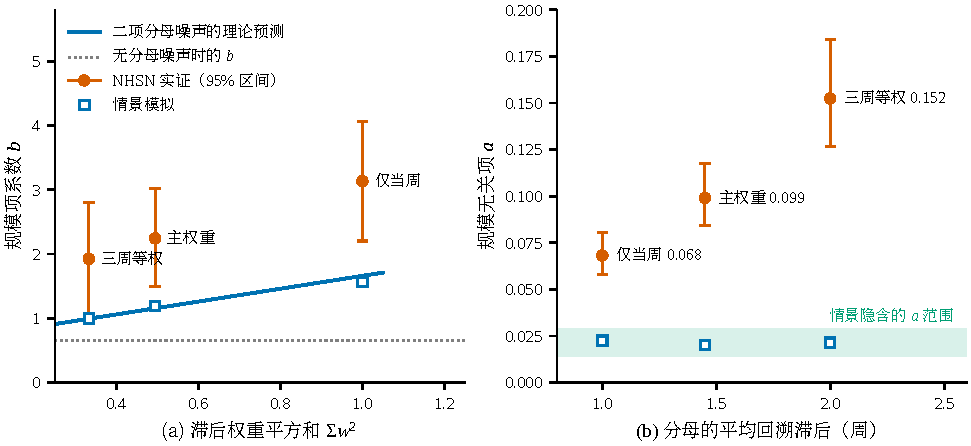
\includegraphics[width=\textwidth]{figures/fig_5_3_denominator_noise.pdf}
  \caption{滞后权重对拟合系数的影响。（a）规模项系数 $b$ 与滞后权重平方和 $\sum w^2$ 的关系。圆点为三种权重的实证估计及 95\% 区间，方块为情景模拟值，斜线为二项分母噪声的一阶近似，水平虚线为没有分母噪声时的 $b$。（b）截距 $a$ 与分母平均回溯滞后的关系，阴影为情景隐含的截距范围 0.014--0.029。}
  \label{fig:noise}
\end{figure}

三种滞后权重下规模项都为正，误差形状稳定。经验交叉点则随权重在 12.6--46.0 之间变化，变化方向由斜率与截距的相反走势共同决定，权重越集中，斜率越大、截距越小，交叉点越大。经验交叉点描述的是 $G_t$ 这一统计量的误差结构，它随规模测度的选择而移动，不能当作 $A/v_R$ 的估计。

\section{达峰期的误差结构}
\label{sec:emp-peak}

\subsection{基准偏移}

流行达峰后，阶段均值本身发生变化。取三个流行季的全国峰值周（2022 年 12 月 3 日、2023 年 12 月 30 日、2025 年 2 月 8 日）及其后 7 周，共 1,220 个州周，平均增长比降到 $\Rbar_{\mathrm{peak}}=0.8075$，标准差 0.3048。平均增长比小于 1，说明住院数在这一阶段平均每周下降约两成。若继续用初期均值 1.6706 作基准，各箱的平均损失都在 0.29--0.31 之间，看不出随规模下降。

在固定基准下，损失可以拆成两块：基准偏移造成的常数偏差，以及箱内围绕峰期均值的波动。常数偏差为
\begin{equation}
  \frac{(\Rbar_{\mathrm{early}}-\Rbar_{\mathrm{peak}})^2}{\Rbar_{\mathrm{early}}^2}=0.2669,
  \label{eq:peak-bias}
\end{equation}
它与规模无关，相当于在式~\eqref{eq:mse-decomp} 的条件偏差项中加入了一个阶段转换的偏移。表~\ref{tab:peak-bins} 与图~\ref{fig:peak} 给出分箱结果。偏差项占总损失的 88.9\%，从最小箱的 59.5\% 升到最大箱的 94.8\%。规模越大，箱内波动越小，偏差项的占比越高。除最小箱外，峰期损失是同箱初期损失的 1.8--2.9 倍；最小箱只有 33 个州周，峰期的小规模州周较少，其比值 0.91 不稳定。

\begin{table}[!tbp]
  \centering
  \caption{达峰期以初期均值为基准时的分箱误差分解}
  \label{tab:peak-bins}
  \small
  \begin{tabular}{@{}lccccccc@{}}
    \toprule
    $D_t$ 分箱 & 州周数 & 总损失 & 偏差项 & 箱内波动 & 偏差占比（\%） & 初期损失 & 峰期/初期 \\
    \midrule
    $[5,20)$ & 33 & 0.300 & 0.178 & 0.122 & 59.5 & 0.329 & 0.91 \\
    $[20,50)$ & 140 & 0.293 & 0.227 & 0.066 & 77.6 & 0.160 & 1.82 \\
    $[50,100)$ & 162 & 0.312 & 0.270 & 0.042 & 86.6 & 0.145 & 2.16 \\
    $[100,250)$ & 312 & 0.305 & 0.276 & 0.029 & 90.5 & 0.112 & 2.73 \\
    $[250,600)$ & 311 & 0.300 & 0.277 & 0.023 & 92.4 & 0.103 & 2.90 \\
    $[600,5000)$ & 262 & 0.292 & 0.277 & 0.015 & 94.8 & 0.105 & 2.77 \\
    \bottomrule
  \end{tabular}

  \vspace{4pt}
  {\small 注：峰期为各季全国峰值周及其后 7 周，共 1,220 个州周；基准为初期均值 1.6706。}
\end{table}


\begin{figure}[!tbp]
  \centering
  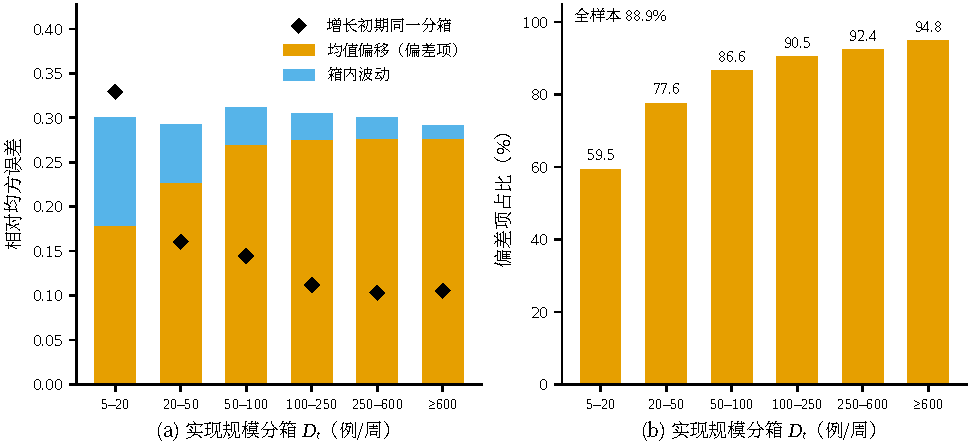
\includegraphics[width=\textwidth]{figures/fig_5_4_peak_decomp.pdf}
  \caption{达峰期（峰值周及其后 7 周）以流行初期均值为基准时的误差分解。（a）各规模箱的平均损失，分为基准偏移造成的偏差项与箱内波动，菱形为同一分箱在流行初期的平均损失；（b）偏差项在各箱损失中的占比。}
  \label{fig:peak}
\end{figure}

\subsection{阶段自身基准下的规模效应}

改用峰期自身均值作基准后，规模效应重新出现，$a=0.0665$（95\% 区间 0.0467--0.0897），$b=7.927$（5.424--11.225），交叉点 119.2（64.0--225.9），平均损失 0.142。峰期的误差仍然呈“常数加规模反比”的形状，规模项在峰期依然有用。

峰期的 $b$ 不能直接与初期的 2.243 比较。式~\eqref{eq:loss} 以阶段均值的平方归一化，峰期均值只有初期的一半左右，归一化分母小了约四倍，斜率因而被机械地放大。统一用 $\Rbar_{\mathrm{early}}$ 归一化后，峰期斜率为 1.852，低于初期的 2.243；不归一化时为 5.169 对 6.261。在同一样本上做联合回归，阶段交互项的普通最小二乘估计为 $-0.92$，95\% 区间 $-2.33$--$0.59$，包含零。因此，达峰期规模仍然有用，但没有证据表明它比初期更有用或更没用。

达峰期结果揭示了误差的另一种来源。阶段转换时，基准的偏移量远大于规模项，用旧基准预测新阶段，规模再大也无法降低误差。监测上的对应做法是换用能够跟踪基准变化的模型，同时继续维持病例规模，前者处理偏差项，后者处理规模项。第六章用时变基准与 FluSight 集成预测考察第一点。

\section{填报制度变化}
\label{sec:emp-policy}

填报制度的变化提供了另一类证据。按命题~\ref{prop:reporting}，报告率下降会增加方差；若填报率下降只是均匀地稀疏了病例，$G_t$ 的离散程度应按可预测的幅度上升。表~\ref{tab:policy} 与图~\ref{fig:policy} 比较三期 $G_t$ 的分布。

从第一期到第二期，$G_t$ 的标准差从 0.624 升到 1.823，增加 192\%；第三期回到 0.649。稳健离散度几乎不动，四分位距依次为 0.638、0.594、0.652，第二期反而略低；中位绝对偏差为 0.298、0.299、0.292。偏度从 3.29 升到 14.98，再回到 2.68；最大值从 12.7 升到 33.9。第 10 百分位数从 0.468 降到 0.199，左尾也在扩张。两端尾部都变厚，而分布中部不变。

\begin{figure}[!tbp]
  \centering
  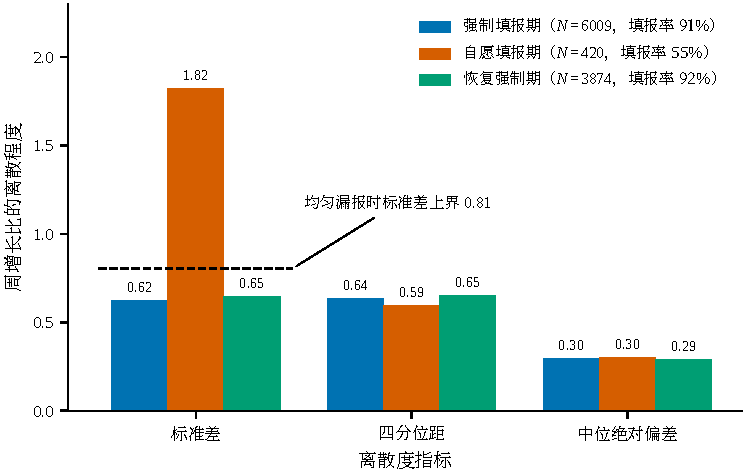
\includegraphics[width=0.8\textwidth]{figures/fig_5_5_reporting_policy.pdf}
  \caption{三个填报制度期内周增长比 $G_t$ 的离散程度。柱上数字为指标值；虚线为填报率从 91.1\% 降至 54.6\% 时，若漏报在医院间均匀发生，第二期标准差可能达到的上限。}
  \label{fig:policy}
\end{figure}

均匀稀疏给出的上限可以直接计算。若填报医院的减少相当于把每家医院的病例按相同比例抽稀，规模缩小到原来的 $54.59/91.11$，按规模项与 $1/m$ 成正比且忽略环境项，标准差最多放大到
\begin{equation}
  0.624\times\sqrt{91.11/54.59}=0.806,
  \label{eq:sd-bound}
\end{equation}
即 1.29 倍。实际放大了 2.92 倍，而且只有标准差放大，分位数指标不变。离散程度的扩张因此来自少数极端周，例如部分医院时报时不报造成的跳变：某周填报医院骤减，住院数随之骤降，$G_t$ 落入左尾；次周恢复填报，$G_t$ 落入右尾。整体噪声并没有均匀增加。第二期缺失的 36 个州周按 0 计入，也会制造这类跳变。

两项对照排除了两个明显的混杂。第二期覆盖 5--10 月，多为非流行季，因此先检查季节构成。只取 10 月至次年 3 月的周，第一期与第三期的标准差为 0.652 和 0.706，第二期（仅 2024 年 10 月，55 个州周）为 4.79，扩张仍然存在，但第二期的样本很少。填报率的连续变化同样不能解释扩张：以 2022 年 10 月 1 日为界把第一期分为两段，平均填报率由 87.8\% 升到 93.7\%，标准差为 0.628 和 0.620，几乎不变。强制填报下填报率的小幅变化不影响离散程度，自愿填报带来的变化是结构性的。

第二期离散度的扩张与命题~\ref{prop:reporting} 只有定性联系。报告率下降确实增加了方差，但第二期的主要变化是填报行为的结构性扰动，无法用 $\rho$ 的变化定量解释。对监测数据质量的评估而言，标准差对这类扰动最敏感，四分位距与中位绝对偏差则反映整体噪声水平，两类指标并用可以区分结构性扰动与均匀漏报。

\section{本章小结}
\label{sec:emp-summary}

本章在美国 51 个辖区的流感住院周报上检验了第三章的误差形状。流行初期 1,267 个州周的相对均方误差随实现规模下降并趋于平缓。可行广义最小二乘估计的截距为 0.0991，斜率为 2.243，所有重抽的斜率都为正。经验交叉点为 22.6 例/周，与理论情景区间 21.3--49.2 处于同一量级。平均损失中截距与规模项大致各占一半。把规模提高到每周 250 例，模型给出的损失下降约四成，此后截距占九成以上。

截距与斜率都是情景隐含值的三倍以上，比值的吻合因此不能作为结构参数的检验。滞后权重的比较表明，分母中的二项报告噪声按 $\sum w^2$ 抬高斜率而不改变截距，其预测的相对变化与实证吻合。二项噪声只能解释斜率水平的一半左右。截距随分母的回溯滞后单调上升，与环境的时间相关和 $G_t$ 的口径一致。经验交叉点随规模测度在 12.6--46.0 之间移动，只能作量级参考。

达峰期以初期均值为基准时，88.9\% 的损失来自基准偏移，规模效应被掩盖；换用峰期自身基准后规模项重新为正，阶段间的斜率差异不显著。自愿填报期 $G_t$ 的标准差扩张 192\%，稳健离散度不变，扩张来自少数极端周，超出均匀稀疏所能解释的幅度。第六章检验这些结论在替代设定、空间汇总与外部数据下是否保持。
